\chapter[Using the diallel to select optimal bi-parental crosses to map QTL]{Using the diallel to select optimal bi-parental crosses to map QTL
\footnote{This chapter represents a mature draft of a manuscript currently in preparation, with slight modifications made for the format. Current author line and title are: Keele, G. R., Maurizio, P. L., Oreper, D., Valdar, W. Diallel-informed experimental cross selection for QTL mapping.}}
\label{chap:didact}

\section{Introduction}

Geneticists commonly conduct experiments with the goal of identifying quantitative trait loci (QTL) using crosses of inbred strains of model organisms. These experiments can be costly in terms of resources, due to the organisms, their care, genotyping or sequencing, as well as the time and energy required for the experiment itself. In the face of these constraints, procedures that explore the potential set of experimental cross designs and allow researchers to select experiments with greater potential to be successful are beneficial to the field of complex traits.

Although the goals for a given experiment will be nuanced and unique to each study, the mapping portion is successful if a QTL is detected with a statistically significant signal, using established methodologies \citep{Lander1989,Haley1992,Dupuis1999,Broman2001}. This outcome is not guaranteed simply due to the presence of segregating QTL in the mapping population: the experimental design may not be sufficiently powered to identify them. The power of an experiment, the probability that a non-zero effect will be recognized given that it is present, is influenced by a number of biological factors, some of which can be more easily manipulated and optimized through experimental design choices. These factors include genetic architecture, mode of action, and the variation in the population due to noise. If the genetic architecture of the trait is highly polygenic with many loci of small effect, power will be reduced compared to tests for QTL of larger effect. Similarly, mode of action (e.g. additive, dominant), for a QTL will also influence power because certain experimental designs will have differential ability to detect a given effect type. For example, a backcross (BC) cannot identify a QTL underlying a fully recessive effect when the homozygote of the recessive allele is never observed. Finally, an increase in variation due to noise will decrease power because the noise drowns out the true signal. Ideally, investigators would select the experiment that can best handle these factors in the given setting.

In the context of crosses of inbred organisms, one major component of the experimental design is the founder or parental strains. The selection of parental strains allows the investigator to control the genetic background of the experimental population, which can greatly influence the previously mentioned biological factors, and ultimately influence the potential for mapping success. For example, a trait could be highly polygenic and have loci with complex modes of action within natural populations, but much of the genetic and phenotypic variation becomes fixed within two closely related inbred strains. The reduced genetic variability can impact all of the biological factors: the complexity or polygenic nature of the genetic architecture by fixing many of the loci, the mode of action by limiting the potential for epistatic effects through less segregating variants, and the variance attributable to noise through the reduction in phenotypic variability. 

The ability to strongly influence the sources of variation in the population is important to consider. If the QTL explains a large proportion of the variance in the population, a simple cross will be well-powered to identify the QTL, even if its effect is small. The balance between the variance attributable to the QTL versus how generalizable the experiment is to natural populations is important to consider when making decisions about experimental design. Ultimately a finding that is characteristic of only a very unnatural experimental population and does not generalize well to more natural, outbred ones, will greatly reduce the impact of such an experiment and even undermine the purpose of experiments of model organism in general. The ideal experiment will be well-powered to identify QTL, but also generalizable to natural populations.

\begin{figure}
\renewcommand{\familydefault}{\sfdefault}\normalfont
\centering
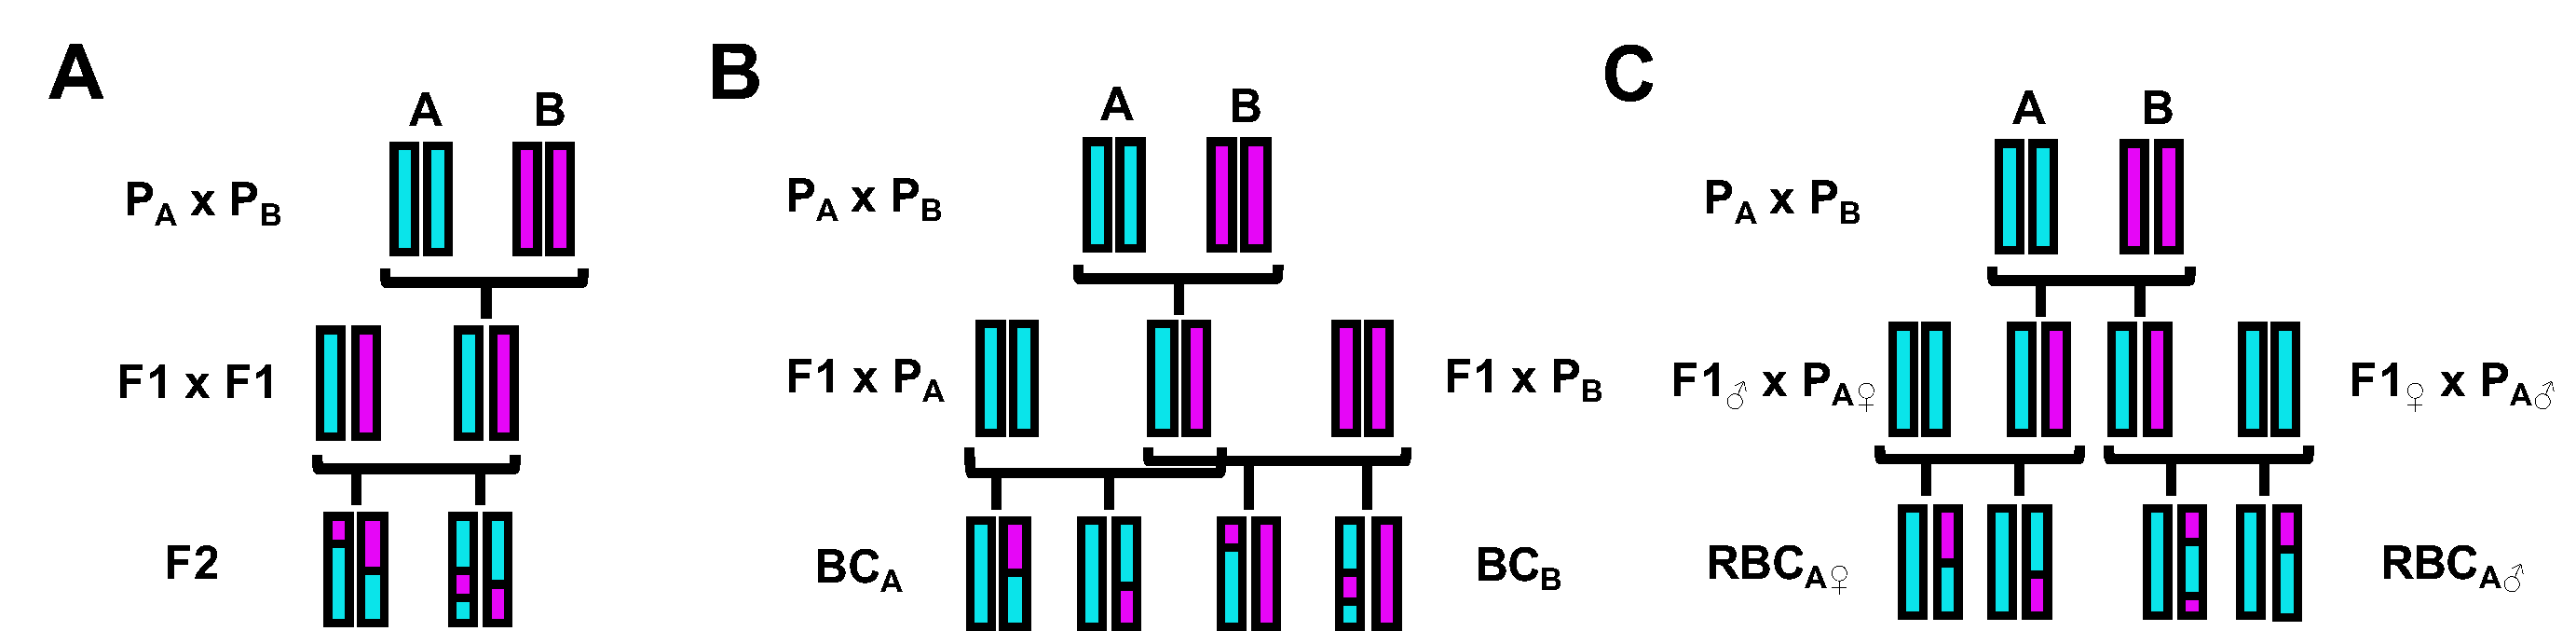
\includegraphics[width=\textwidth]{figures/2-didact/biparental_crosses.pdf}
\caption[Diagrams of bi-parental crosses]{Diagrams of potential bi-parental crosses that we consider with DIDACT: F2 (A), BC (B), and RBC (C). An parental haplotype is represented as a single colored chromosome. The P and F1 generations are replicable, whereas the mapping populations are not. Of these three cross designs, only the F2 mapping population has potentially all three genotypes at a locus (A/A, A/B, and B/B), which allows for additive and dominance effects to be estimated. With traditional BC, one parental homozygote is possibly observed, depending on which parent is back crossed. By jointly analyzing RBC, it is possible to detect effects from heterozygous sites in which the parent-of-origin differs for the back crossed parental allele.\label{fig:biparental_crosses}}
\end{figure}

% Pilot data

The power of an experiment cannot be directly assessed because it requires knowledge of the true effect, which is unknown. Instead power calculations are performed for a range of plausible parameters, usually over varying effect sizes or sample sizes, given some type I error level and error variance, which can then be represented as power curves. Power calculations have been specifically developed and refined for simple cross designs such as F2 intercross, BC, and recombinant inbred (RI) strain panels, using an information perspective approach, which posits that the complete information is composed of the observed information and the missing information \citep{Sen2005}. These power calculations are still dependent on assumed parameters, in this case QTL effect sizes and error variances. As a result, meaningful and useful power calculations still depend on the consideration of an appropriate set of values for these unknown quantities, otherwise the power estimates could be uninformative or even misleading.

% F0 and F1
% Estimation of additive, inbred, and epistatic effects

Pilot data can provide information about the underlying genetic signals present in potential experiments. One  source of pilot data is the inbred founder strains themselves as well as their hybrid crosses (F1). Comparisons of F1 individuals to the inbred strains can provide estimates of various genetic effects for given strains, aggregated from causal variants across the entire genome. These effects can include additive, inbred, and epistatic. An additive effect for a given strain can be estimated from averages of F1 that do not have the strain as a parent (0 copies), to averages of F1 that do have the strain as a parent (1 copy), and finally to the inbred strain itself (2 copies). An inbred effect is estimated from these same sets of crosses, but represent the average departures observed from the expectation of the hybrid according to the additive effect to its actual observed value. An epistatic effect represents departures from expectation for a specific cross of two strains, thus it is an interaction effect of the two strains.

% Reciprocal crosses

Additional information is contained in the reciprocal crosses that compose the F1 hybrids, and can be characterized as parent-of-origin effects (POE). Reciprocal F1 crosses have the same parental strains, but the dam-sire identities are switched. The average differences between reciprocal crosses can be used to estimate the POE. QTL underlying these POE effects can be mapped using a unique BC design that we will refer to as RBC \citep{Gonzalo2007}. RBC subtly differs from what is traditionally known as reciprocal BC, in which the F1 is the same but back crossed to the alternative parental strain. RBC have the same F1 and back crossed parent, but the dam and sire strains are reversed between reciprocal pairs; thus the parent-of-origin for each allele is known at heterozygous sites, and differences in the trait that correlate to genotype and parent-of-origin can be detected. The estimation of POE through reciprocal crosses allows researchers to add RBC to their collection of potential experiments. Though RBC are not as commonly used as F2 and BC, interest in POE has increased \citep{Lawson2013,Berenos2014a,Connolly2014,Harper2014a,Zou2014}. Pilot data that distinguishes between reciprocal F1s allow for an even larger number of experiments to be explored and considered. These potential bi-parental mapping populations, F2, BC, and RBC, are depicted in \textbf{Figure \ref{fig:biparental_crosses}}.

% Diallel

These experiments can best be explored with the full set of potential founder lines and their F1 hybrids, which represent a classic genetic experiment, the diallel. Diallel crosses have been performed in a number of traits and across a diverse set of organisms, including mating speed, female receptivity, and temperature preference in fruit fly \citep{Parsons1964,Casares1992,Yamamoto1994}; immune function, polyandry, and genetic-environment interactions in crickets \citep{Rantala2006,Ivy2007,Nystrand2011}; and heterosis and reciprocal effects in poultry \citep{Emsley1983}. Additionally, the diallel has a long history in plant breeding \citep{Gilbert1958} and numerous recent applications \citep{Bahari2012,GhareebZeinab2014,DosSantos2016}. 

Since being described in the early 20\textsuperscript{th} century, statistical methodology for the diallel has seen steady advancements, from estimating the general combining ability with related F2 populations \citep{Griffing1956}, the use of random effects \citep{Zhu1996,Tsaih2005}, and the use of a Bayesian hierarchical model for a sparse diallel \citep{Greenberg2010}. Recently, \cite{Lenarcic2012} used Bayesian hierarchical modeling of diallel data to allow for stable estimation of a large number of strain-level genetic effects (such as additive, inbred, epistatic, and maternal), and has been used to analyze a number of phenotypes and organisms, such as cranial shape \citep{Gonzalez2016}, response to treatment and infection \citep{Crowley2014,Maurizio2017} in mice, and shoot growth in carrots \citep{Turner2017}. Even incomplete or sparse diallel data can be used for the characterization of some of the underlying strain-level genetic signals, which can then be used to evaluate the potential space of experiments, and allow for the selection of a favorable one. A simplified representation of a diallel, in the founders of the Collaborative Cross (CC), a multiparental recombinant inbred panel in laboratory mouse, is shown in \textbf{Figure \ref{fig:cartoon_diallel}}.

\begin{figure}
\centering
\includegraphics[width=0.6\textwidth, page=4, trim={1in 0in 3in 0in}, clip]{figures/2-didact/mapping_crosses.pdf}
\caption[Diagram of the diallel]{A cartoon representation of a diallel of the CC founders. Each unique strain genome is represented as a single colored chromosome. Genomes along the diagonal represent the inbred founders themselves. Off-diagonal genomes are the F1 hybrids of a pair of founders. Mirrored genomes across the diagonal represent reciprocal F1 genomes, in which the genotypes will be identical, but parent-of-origin for each chromosome will be flipped. All the genomes in a diallel are replicable, and can thus be measured on multiple individuals. Some cells of the diallel may not be observed, which reduces the ability to estimate certain strain effects. \label{fig:cartoon_diallel}}
\end{figure}

% Put it altogether

\cite{Verhoeven2006} investigated jointly modeling diallel data with the related downstream F2 populations, and found that it allowed for the simultaneous dissection of the trait across all the populations, or characterization of strain-level effects, as well as the ability to generalize the QTL findings from the mapping populations in terms of the multiparental diallel population. We focus on the situation in which none of the F2 populations, or any such downstream cross populations, are observed, and attempt to evaluate the utility of potential crosses in terms of QTL mapping. Herein we bring together three lines of research: 
\begin{enumerate}
	\item The estimation of the power to map putative QTL of given effect sizes.
	\item The characterization of genetic effects from pilot data.
	\item The selection of optimal experiments through a decision theoretic approach.
\end{enumerate}
We use a Bayesian hierarchical model to characterize the genetic information contained in pilot data as aggregate strain effects \citep{Lenarcic2012}. This Bayesian approach allows us to stably estimate a large number of genetic effects through the sharing of information across strains, as well as assess the uncertainty around these effects. This uncertainty is then propagated through to power calculations of potential experimental crosses, which is generally ignored in power calculation and experiment selection. Our approach will aid researchers in selecting better experiments with greater potential according to pilot data over ineffective or inefficient options. These opportunities include not only favorable experiments for mapping additive traits, which have commonly been studied, but also for mapping the QTL responsible for less well-understood effects such as POE.

\section{Statistical Models and Methods}

Our approach builds on three separate areas of research. Firstly we consider the calculation of power to map QTL given that the QTL effect $\theta$ is known. This will require the review of general concepts in quantitative genetics and statistics in the context of crosses of two inbred strains. Because in reality $\theta$ is never actually observed, we next consider the characterization of $\theta$ from pilot data. Finally we discuss the selection of optimal experimental crosses through the maximization of a chosen utility function.

% Power
\subsection{Power to map QTL}

\subsubsection{Single QTL model of bi-parental cross} 

Here we review the general concepts in quantitative genetics and statistics that support the method used by \cite{Sen2005} for power calculations of traditional crosses like the F2 and BC. Consider this model:
\begin{equation}
	y_{i} = \qtl_{i} + G_{i} + E_{i} + \epsilon_{i}
    \label{eq:general_model}
\end{equation}
where $y_{i}$ is the phenotype of individual $i$, $\qtl_{i}$ is the effect of the QTL for individual $i$, $G_{i}$ is the effect of other genetic elements for individual $i$, $E_{i}$ is the effect of environmental factors for individual $i$, and $\epsilon_{i}$ is the random noise for individual $i$. $G_{i}$ and $E_{i}$ are un-modeled, and can thus be collapsed with $\epsilon_{i}$ into a single error term $\varepsilon_{i}$.
\begin{equation}
	y_{i} = \qtl_{i} + \varepsilon_{i}
    \label{eq:reduced_model}
\end{equation}
where $\varepsilon_{i} \sim \text{N}(0, \sigmasq)$ with $\sigmasq$ representing the error variance in the data. The QTL effect is a vector, traditionally parameterized as additive and dominant effects \citep{Lynch1998}. This can be formulated in a traditional regression framework:
\begin{align}
	\by &= \bX\bbeta + \bepsilon \label{eq:linear_model} \\ 
	&= \bX \left[\begin{array}{c}\mu \\ \alpha \\ \delta \\ \end{array}\right] + \bepsilon \nonumber,
\end{align}
where $\by$ is the phenotype vector, $\bX$ is the design matrix that we will define further, $\bbeta$ is the vector of effects composed of $\mu$, the overall phenotypic mean, $\alpha$, the additive effect of the QTL, and $\delta$, the dominance effect for the QTL, and $\bepsilon$ is the vector of errors. Consider an F2 or BC of strains $A$ and $B$, with the genotype of an individual represented in terms of strain identity, denoted in the subscript. $\alpha$ is the midpoint of the difference between the homozygotes:
\begin{equation}
	\alpha = \frac{\text{E}(y_{AA}) - \text{E}(y_{BB})}{2}
    \label{eq:additive}
\end{equation}
 $\delta$ is the deviation of the heterozygote from the average of the homozygotes:
 \begin{equation}
 	\delta = \text{E}(y_{AB}) - \frac{\text{E}(y_{AA}) + \text{E}(y_{BB})}{2}
    \label{eq:dominance}
\end{equation}
\textbf{Table \ref{tab:qtl_mean_model}} lists Eq \ref{eq:linear_model} parameterized in terms of these QTL effects. This parameterization maintains the identifiability of all the effects, though it may not be as intuitive to researchers accustomed to more traditional regression models used commonly in genome-wide association studies.

\begin{table}
\renewcommand{\familydefault}{\sfdefault}\normalfont
\begin{minipage}{\textwidth}
%\captionsetup{width=\textwidth}
\centering
\caption{Model of QTL effect on the mean for F2 and BC
\label{tab:qtl_mean_model}}
\end{minipage}
\begin{minipage}{\textwidth}
\begin{tabularx}{\textwidth}{XXXXXX}
\hline
%\header
& & & \multicolumn{3}{c}{Probability\footnote{Mendelian inheritance probabilities based on independent assortment of alleles $A$ and $B$ for specified bi-parental cross.}} \\ \cline{4-6}
%\header
Genotype & 
$\text{E}(y)$\footnote{Parameters as defined in Eq \ref{eq:linear_model}, Eq \ref{eq:additive}, and Eq \ref{eq:dominance}.} & 
$\bx$\footnote{Row vector of the design matrix $\bX$ in Eq \ref{eq:linear_model}.} 
& F2 & BC$_{A}$ & BC$_{B}$ \\
\hline
AA & $\mu + \alpha - \frac{\delta}{2}$ & $\left[\begin{array}{ccc} 1 & 1 & -\frac{1}{2}  \end{array}\right]$ & $\frac{1}{4}$ & $\frac{1}{2}$ & $0$ \\
AB & $\mu + \frac{\delta}{2}$ & $\left[\begin{array}{ccc} 1 & 0 & \frac{1}{2}  \end{array}\right]$ & $\frac{1}{2}$ & $\frac{1}{2}$ & $\frac{1}{2}$ \\
BB & $\mu - \alpha - \frac{\delta}{2}$ & $\left[\begin{array}{ccc} 1 & -1 & -\frac{1}{2}  \end{array}\right]$ & $\frac{1}{4}$ & $0$ & $\frac{1}{2}$ \\
\hline
\end{tabularx}
\end{minipage}
\end{table}

Returning to the formulation of the model in Eq \ref{eq:variance}, the variance of the model can be characterized as follows with the assumption that there is no covariance between the QTL effect and the error,
\begin{equation}
	\text{Var}(y) = \text{Var}(\text{QTL}) + \sigmasq
    \label{eq:variance}
\end{equation}

The background genetic and environmental variation are captured in $\sigmasq$; here we focus on the variability due to the QTL. $\text{E}(y)$ will vary depending on the genotype, which will vary probabilistically according to the type of cross, as described in \textbf{Table \ref{tab:qtl_mean_model}}. As example, for an F2 cross, the $\text{Pr}(AA) = \frac{1}{4}$, $\text{Pr}(AB) = \frac{1}{2}$, and $\text{Pr}(BB) = \frac{1}{4}$. The variance of a random variable $X$ is defined as $\text{Var}(X) = \text{E}(X - \text{E}(X))^{2}$. The variable $X$ in this setting is QTL, which is the categorical genetic state at the QTL. The expectation of $X$ is $\text{E}(X) = \sum_{x \in \mathcal{X}}x\text{Pr}(X=x)$. Based on the genotype probability for a given cross, the variances due to the QTL in terms of the QTL effects are presented in \textbf{Table \ref{tab:qtl_variance_model}}.

\begin{table}
\renewcommand{\familydefault}{\sfdefault}\normalfont
\begin{minipage}{\textwidth}
%\captionsetup{width=\textwidth}
\centering
\caption{Variance attributable to QTL effect for F2 and BC
\label{tab:qtl_variance_model}}
\end{minipage}
\begin{minipage}{\textwidth}
\begin{tabularx}{\textwidth}{XXXXX}
\hline
%\header
Model & 
Parameter\footnote{Parameters as defined in Eq \ref{eq:linear_model}, Eq \ref{eq:additive}, and Eq \ref{eq:dominance}.} & 
F2 & BC$_{A}$ & BC$_{B}$ \\
\hline
General & & $\frac{1}{4}\delta^{2} + \frac{1}{2}\alpha^{2}$ & $\frac{1}{4}(\alpha + \delta)^{2}$ & $\frac{1}{4}(\alpha + \delta)^{2}$ \\
Fully additive & $\delta = 0$ & $\frac{1}{2}\alpha^{2}$ & $\frac{1}{4}\alpha^{2}$ & $\frac{1}{4}\alpha^{2}$ \\
A dominant & $\delta = \alpha$ & $\frac{3}{4}\alpha^{2}$ & $0$ & $\alpha^{2}$ \\
B dominant & $\delta = -\alpha$ & $\frac{3}{4}\alpha^{2}$ & $\alpha^{2}$ & $0$ \\
Fully dominant & $\alpha = 0$ & $\frac{1}{4}\delta^{2}$ & $\frac{1}{4}\delta^{2}$ & $\frac{1}{4}\delta^{2}$ \\
\hline
\end{tabularx}
\end{minipage}
\end{table}

The mode of action of the locus impacts the variability in phenotype due to QTL within a cross type, as seen in \textbf{Table \ref{tab:qtl_variance_model}}. This is particularly noticeable in the BC experiments, where certain modes of action produce no variance. If the locus is recessive (or conversely dominant), the genotype with differing phenotype will not be observed, and nor will variation due to QTL. Finally, cross type also impacts the QTL variance, which is also clear in \textbf{Table \ref{tab:qtl_variance_model}}. Increasing the variance attributable to the QTL will increase power to map the QTL; in contrast, increasing the overall variance that is attributable to noise (un-modeled background genetic factors or environmental factors) will reduce the significance of statistical tests, and thus decrease the power.

% Power calculation

\subsubsection{Power calculations} 

Analytical power calculations are generally based upon some null distribution for a statistic of interest as well as some range of values for the statistic that will be observed in the experiment. Consider $\theta$, some function of the QTL effects $\alpha$ and $\delta$, as the parameter of interest. We wish to calculate the probability of mapping the QTL that results in $\theta$. In terms of the association modeling, a natural null hypothesis is $H_{0}: \theta = \theta_{0}$ with $\theta_{0} = 0$, that there is no QTL effect. The alternative hypothesis is $H_{A}: \theta \neq \theta_{0}$. By specifying a model for the data, or more precisely the distribution of the error term of the model, the likelihood $\mathcal{L}(\theta)$ can be evaluated. The likelihood ratio test (LRT) statistic, $T = -2\log\frac{\mathcal{L}(\theta = 0)}{\mathcal{L}(\theta = \widehat{\theta})}$, where $\widehat{\theta}$ is a proposed estimate of $\theta$, can be used to perform power calculations. 

To use the LRT statistic for power calculations, a significance threshold and corresponding statistic distribution for $T$ are necessary. The traditional scale of significance used in the linkage and QTL fields is the $\log_{10}$ likelihood ratio or LOD (logarithm of odds) score. Historically a LOD score of 3 ($2\log(10) \times 3$ on the likelihood ratio scale) has been used as a significance threshold, meaning approximately that the data support the alternative model over the null model 1000 to 1. A more stringent significance threshold than 3 can be used to further reduce the risk of false positives or possibly account for a multitude of tests (though it is worth noting these tests will not be fully independent). Given some significance threshold $C$ is chosen to determine genome-wide significance; if $T \ge C$ for some locus, the null hypothesis is rejected. The threshold $C$ will affect the the true positive and false positive rates, and more important to our topic, the power.

Statistically, power is the probability that the null hypothesis is rejected given that alternative hypothesis is true. The LRT $T$ is the statistic upon which the power calculations are drawn, thus the power will be $\text{Pr}(T \ge t | \theta \neq \theta_{0})$ where $t$ is the observed statistic produced by the data. With the LRT statistic, when the models are nested and the maximum likelihood estimate (MLE) is used ($H_{A}: \theta = \widehat{\theta}_{\text{MLE}}$), as they are in this case, and the null model is true, $T$ is asymptotically $\chi^{2}_{k}$ distributed, where $k$ is the degrees of freedom, the difference in number of parameters between the models. A power calculation from this distribution would not be useful because it would represent the probability that the null hypothesis is rejected when there is no genetic effect, or the false positive probability. The power is rather based on the alternative hypothesis being true, $\theta \neq \theta_{0}$, and thus $\chi^{2}_{k}$ distribution is inappropriate. When the alternative hypothesis is true rather than the null, that $\theta = \widehat{\theta}_{\text{MLE}}$, $T$ is proportional to the noncentral $\chi^{2}$ distribution with noncentrality parameter $(\theta - \theta_{0})^{T}\mathcal{I}(\theta)(\theta - \theta_{0})$ where $\mathcal{I}(\theta)$ is the expected Fisher information matrix. We model the data with a Gaussian mixture distribution with a shared residual variance, which naturally extends from the bi-parental cross statistical model. A key feature of this model is that the LRT reduces to the variance attributable to the QTL as a function of effects that we presented in table 1. This variance parameter is scaled by $\sigmasq$, which sets the variance of each Gaussian component to 1. Thus the power calculations are intuitively a function of the effect size, the proportion of the variance explained by the QTL (effect size combined with residual error variance), and the sample size.

It is important to note that the actual $\widehat{\theta}_{\text{MLE}}$ cannot be calculated because no actual cross data for QTL mapping is observed, but the underlying theory of the method assumes that the alternative $\theta$ is the MLE estimator. $\sigmasq$ is also never actually known, but we estimate it from the information present in the pilot data. The final interpretation of this power calculation is the probability that a significant result is found ($T \ge t$) given that there is some QTL effect specified in the proposed MLE estimator $\widehat{\theta}_{\text{MLE}}$ with an error variance of $\sigmasq$.

\cite{Sen2005} develop the theory further to account for the fact that the information is generally never complete in QTL studies. The true QTL variant is most likely not observed (genotyped), but rather loci in linkage disequilibrium are, and thus contain some of the information from the QTL. They develop the theory to take into account this missing information from sparse markers (as previously described), as well as selective genotyping (genotyping study individuals on the tails of the phenotype distribution). As a result of this, power can be reduced by not only greater error variance, but also missing information. The advancement in genotyping technology is generally leading to denser markers in QTL studies, leading us to make the assumption of complete information. We directly incorporate the R package qtlDesign \citep{Sen2007} into our method, so missing information can be specified in the power calculations. See \cite{Sen2005} for a description of the missing information theory used.  

% Bayesian hierarchical model

\subsection{Characterization of strain-level genetic effects from pilot data}

The power calculations described above are dependent on known QTL effects $\theta$, but in reality, $\theta$ is not observed. However, information about $\theta$ is contained in pilot data, which can be exploited to characterize plausible distributions for $\theta$. 

\subsubsection{Bayesian modeling of diallel data}

One potential convenient source of pilot data are the parental strains and some subset of their F1 hybrids. Direct estimation of $\theta$ is not possible because no recombinations occur between the parental haplotypes within F1 individuals, but rather strain effects that represent the accumulated effect of the segregating variants within each inbred strain can be estimated. Denote these strain effects, the vector of effects that will be defined in Eq \ref{eq:bayesdiallel}, as $\bphi$ to distinguish them from $\theta$, the effect of a single QTL. 

The strain-level vector $\bphi$ can encompass effects of different modes of actions based on the strain identities of the dam and sire of an individual. These strain-level effects include additive, inbred, epistatic, and maternal. The additive effects characterize the average effect of a strain constrained to a dosage-like model. Such a simple model is not always sufficient to accurately model data, such as the situation that an F1 hybrid is not approximately the midpoint between the parental strain phenotypes. We account for this potential deviation from additivity with an inbred effect, which is in contrast to the more traditional view of non-additivity as dominance. This parameterization of the model is appropriate for our pilot data because, considering $J$ parental strains, there will be $J(J-1)$ possible F1 hybrids, and only $J$  inbreds. When $J$ is greater than 2, which is likely, the number of possible hybrid F1 will outnumber the $J$ strains. Thus modeling the state of being outbred as the default state more intuitively matches the structure of our data.

Epistatic and maternal effects represent other potential sources of deviation from strict additivity. Epistatic effects are essentially an interaction between strains, thus allowing a specific F1 hybrid to deviate from its additive expectations. Maternal effects can capture strain-specific POEs where there is an average difference between reciprocal F1. As demonstrated in \cite{Lenarcic2012}, consider pilot data that are some subset of the $J$ inbred strains and their F1. The strain identities of dam, sire, and dam-sire pair for individual $i$ are indexed as $j[i]$, $k[i]$, and $(j,k)[i]$, respectively. We model the pilot data as
\begin{equation} \label{eq:bayesdiallel}
	y_{i} = \mu + \underbrace{a_{j[i]} + a_{k[i]}}_{\text{additive}} + \underbrace{I_{\{j=k\}}(b_{j} + \beta_{\text{inbred}})}_{\text{inbred}} + \underbrace{I_{\{j \neq k\}}v_{(j, k)[i]}}_{\text{epistatic}} + \underbrace{m_{j[i]} - m_{k[i]}}_{\text{maternal}} + \varepsilon_{i},
\end{equation}
where $y$ is the continuous phenotype value, $\mu$ is the intercept, $a$ is a strain-specific additive or dose effect, $\beta_{\text{inbred}}$ and $b$ are respectively a general inbred effect and a strain-specific inbred effect that are included only if individual $i$ is inbred, $v$ is a strain-by-strain interaction effect that we will call an epistatic effect and is only included if individual $i$ is outbred, $m$ is a strain-specific maternal effect, and $\varepsilon_{i}$ is the individual-specific noise (deviation from the model expectation) and is distributed: $\varepsilon_{i} \sim \text{N}(0, \sigmasq)$. The model can also include important covariates, such as sex, that need to be adjusted for as fixed effects. The complete set of founder strains and all their reciprocal F1 hybrids represent what is called a diallel, which would allow for the estimation of the full set of strain effects described. Although an incomplete diallel cannot estimate all the strain effects, it still provides information that can be used to estimate $\bphi$.

\subsubsection{Prior specification}

Following the lead of \citep{Lenarcic2012}, we use conjugate priors for the parameters in the model. For example, the strain-level additive effects are distributed following $a \sim \text{N}(0, \tau_{a}^{2})$. For fixed effect terms, such as $\beta_{\text{inbred}}$, $\tau^{2}$ is set to $10^{3}$. For the variance parameters, consider $\sigma^{2}$ which is distributed following $\sigma^{2} \sim \text{IG}(\nu/2, \psi/2)$. We set the hyper parameters $\nu$ and $\psi$ to 0.02 and 2 respectively. These represent diffuse priors, with the intention of allowing the information in the data to inform the estimates. The hyper parameter values can be adjusted within DIDACT.

\subsubsection{Strain-level effect to QTL effect}

Transitioning from strain-level genetic effects $\bphi$ to the effect of a single QTL $\theta$ requires some strong assumptions. Pilot data consisting solely of F1 individuals cannot provide information about specific loci or the number of loci contributing to a strain effect; there are an infinite number of genetic architectures that can explain a given strain effect. It is possible that conducting a small set of F2 crosses and investigating the variability in phenotype for the resulting population could provide information about the trait genetic architecture, such as distinguishing between highly polygenic and oligogenic traits, but here we focus on using only F1. We make the assumption that the strain effects represent the effect of a single QTL, which is somewhat biologically unlikely but provides a straightforward approach to connect information in the pilot data to the power calculations. We use Eq \ref{eq:bayesdiallel} to produce expected phenotype values for a given cross of two strains, assuming the trait is controlled by a single QTL. Consider comparing strains $A$ and $B$, Eq \ref{eq:bayesdiallel} produces $\text{E}(y_{AA})$, $\text{E}(y_{AB})$, and $\text{E}(y_{BB})$. From these expected values, we can estimate traditional single QTL additive and dominant effects, $\alpha$ and $\delta$ respectively, using Eq \ref{eq:additive} and Eq \ref{eq:dominance}. These estimates along with estimates of $\sigmasq$ can then be used with the power calculation machinery described before. Different QTL effects will be estimated from the model in Eq \ref{eq:bayesdiallel} for different potential crosses of inbred strains. 

% Decision theory

\subsection{Decision theoretic approach} 

Different inbred strains will possess differing segregating variants to potentially identify. We use our model of pilot data to make predictions for some set of possible experiments, which can be viewed from a decision theoretic \citep{Raiffa2000} perspective as a decision space. Let us define $\mathcal{A}$ as the set potential experimental crosses. Considering $n$ inbred strains, $\mathcal{A}$ could contain all of or some subset of the ${n \choose 2}$ potential F2 crosses and $3n(n - 1)$ potential BC. 

\begin{figure}
\renewcommand{\familydefault}{\sfdefault}\normalfont
\centering
\includegraphics[width=\linewidth, page=8, trim={0in 0in 0in 0in}, clip]{figures/2-didact/mapping_crosses.pdf}
\caption[Illustration of DIDACT]{Illustration of the Bayesian hierarchical model that is fit within DIDACT, and then propagated through to a utility function. The diagram represents a single sample from a Gibbs sampler, though our decision theoretic approach would be compatible generally with other MCMC procedures. Strain-level effects are sampled based on the pilot diallel data, collectively referred to as $\bphi$. A sample of $\bphi$ is then mapped using functions that draw from Eq \ref{eq:additive} and Eq \ref{eq:dominance} and \textbf{Tables \ref{tab:qtl_mean_model}} and \textbf{\ref{tab:qtl_variance_model}} to $\theta|\mathfrak{a}$, with $\theta$ representing the effect of a single putative QTL in a bi-parental cross and $\mathfrak{a}$ a specific type of cross of two specific founder strains. We collectively refer to all $\theta$ from the possible F2 crosses as $\Theta|\text{F2}$, as well as for BC and RBC. Effectively $\Theta$ are functions of $\bphi$, which are then used as inputs into the utility function $u(.)$, in our case, a putative QTL power estimate. This process is repeated for $s$ samples from the MCMC procedure, which allows for posterior estimates on utility.\label{fig:didact_process}}
\end{figure}

\subsubsection{Power as utility function}

Let an element of $\mathcal{A}$ represent a specific action $\mathfrak{a}$, in this setting, a cross experiment that has corresponding single QTL effect composed of $\alpha$ and $\delta$. If we define $Q$ to be a binary variable that the QTL that causes $\theta$ ($\alpha$ and $\delta$) is successfully mapped: $$Q: \begin{cases} q=1 & \text{QTL is mapped} \\ q=0 & \text{QTL is not mapped} \end{cases}$$ $\text{Pr}(Q=1|\mathfrak{a})$ represents the power that the QTL is successfully mapped, and can be calculated using the noncentral $\chi^{2}$ distribution described previously. We next define $\mathcal{C}$ to be the consequence or experiment outcome space for a QTL mapping experiment, where $c =\{q_{1}, \hdots q_{p}\}$ is the specific joint mapping outcome of the $p$ QTL that the cause the strain effects. This step generalizes the problem to multiple QTL rather than a single one, thus allowing us to reduce the assumption of a single QTL causing the strain effect.

A utility function is an important concept in decision theory. It provides a common scale to compare potential experimental outcomes, and select optimal experiments. Alternative utility functions can be devised and easily swapped to place value on differing aspects that investigator want to prioritize.  We define a utility function, $u(.)$, to map from $\mathcal{C}$ to the reduced utility space, $\mathcal{U}$, which we pose as a function of power, a natural quantity to prioritize. Consider the probability of a specific consequence, which will be a product of a function of the individual power for each QTL: $\text{Pr}(c=\{q_{1}, \hdots, q_{p}\}|\mathfrak{a}) = \prod_{i=1}^{p}\text{Pr}(Q_{i} = q_{i}|\mathfrak{a})$.
We define $u(.)$ to be the count of $p$ QTL that were successfully mapped: $u(c) = \sum_{i=1}^{p}q_{i}$. The probability of a utility $\upsilon$ can be calculated from subsets of $\mathcal{C}$:
\begin{align} 
	\text{Pr}(\upsilon|\mathfrak{a}) &= \sum_{c \in \mathcal{C} : \upsilon = u(c)}\text{Pr}(c|\mathfrak{a}) \\ 
    &= \sum_{c \in \mathcal{C}}I_{\{\upsilon = u(c)\}}\text{Pr}(c|\mathfrak{a}) \nonumber
    \label{eq:utility}
\end{align}
Strictly speaking, the probability of a utility is also dependent on QTL effect $\theta$: $\text{Pr}(\upsilon|\mathfrak{a}, \theta) = \sum_{c \in \mathcal{C}}I_{\{\upsilon = u(c)\}}\text{Pr}(c|\mathfrak{a},\theta)$. $\theta$ can be marginalized out through integration: $\text{Pr}(\upsilon|\mathfrak{a}) = \int_{\theta}\text{Pr}(\upsilon|\mathfrak{a}, \theta)\text{Pr}(\theta|\mathcal{D})d\theta$, where $\mathcal{D}$ represents the pilot data.The probability of this utility function provides an evaluation of the uncertainty of mapping QTL of a given effect size, but does not take into account the uncertainty of $\alpha$, $\delta$, and $\sigma^{2}$, which are produced from the Bayesian model. Through Gibbs sampling or some other Markov Chain Monte Carlo (MCMC) method, a Bayesian model can produce $S$ draws from the posterior distribution of these parameters. Monte Carlo (MC) averaging allows us to take into account this extra source of variability, resulting in the posterior expected utility for cross $\mathfrak{a}$:
\begin{align}
	\text{PEU}(\mathfrak{a}) &= \int_{\theta} \int_{\upsilon} \upsilon \text{Pr}(\upsilon|\mathfrak{a}, \theta)d\upsilon d\theta \\
	&= \int_{\theta} \sum_{\upsilon \in \mathcal{U}} \upsilon \sum_{c \in \mathcal{C}}I_{\{\upsilon = u(c)\}}\text{Pr}(c|\mathfrak{a},\theta)d\theta \nonumber
    \label{eq:peu}
\end{align} 
where $\theta$ is the vector function of $\alpha$, $\delta$, and $\sigma^{2}$. The quantity $\sum_{\upsilon \in \mathcal{U}}\upsilon\text{Pr}(\upsilon|\mathfrak{a}, \theta)$ within the $\text{PEU}(\mathfrak{a})$ is the expected utility for a single draw $s$ from the Bayesian model. This quantity is then be averaged over the QTL effect space of the posterior distribution, traversed through the MC samples. This can be summarized as a point estimate such as the posterior mean or median, or the posterior distribution of expected utilities can be plotted for a given cross $\mathfrak{a}$. Interpretations of the $\text{PEU}(\mathfrak{a})$ will vary amongst utility functions, but we will focus our discussions on power as the utility being maximized.

If we assume all $p$ QTL have the same effect size, our utility function $u(c)$, the number of $p$ QTL that were successfully mapped, follows a binomial distribution. Consider simple case of a single QTL ($p$ = 1), in which the binomial reduces to the Bernoulli distribution. In this setting, the $\text{PEU}(\mathfrak{a})$ reduces to the posterior probability of mapping the QTL. When $p$ is greater than one, as with a binomial variable, $\text{PEU}(\mathfrak{a})$ now represents the expected number of QTL to be mapped. Our approach should be flexible to any reasonable utility function investigators can define, but we emphasize power because its $\text{PEU}(\mathfrak{a})$ are easy to interpret.

\subsection{Availability of data and software}

All analyses were conducted in the statistical programming language R \citep{RSoftware2018}. Our R package DIDACT (Diallel Informed Decision theoretic Approach for Crosses Tool), which is available on GitHub at \url{https://github.com/gkeele/DIDACT}, can estimate strain-level effects from diallel data using a Bayesian hierarchical model, and then perform the posterior utility analysis. The R package BayesDiallel can alternatively be used to estimate the strain-level effects, and used as inputs to DIDACT.

DIDACT includes three diallel data sets from the CC founders \citep{Churchill2004,Hall2012,Srivastava2017}, each with a number of phenotypes, described in detail in \cite{Lenarcic2012}. The CC founders represent the following inbred strains of mouse (abbreviated names in parentheses): A/J (AJ), C57BL/6J (B6), 129S1/SvImJ (129), NOD/LtJ (NOD), NZO/H1LtJ (NZO), CAST/EiJ (CAST), PWK/PhJ (PWK), and WSB/EiJ (WSB).

We also make use of an additional diallel data set in the CC founders of response to Influenza A virus (IAV) infection phenotypes, and is available at \url{https://github.com/mauriziopaul/flu-diallel}.

\section{Results}

We provide example analyses from diallel data of the CC founders to demonstrate our decision theoretic procedure used in the DIDACT package. Our approach depends on assumptions about the effect of a single putative QTL in a bi-parental cross (described in \textbf{Table \ref{tab:qtl_mean_model}}) given strain-level effects estimated from diallel data based on the parameterization described in Eq \ref{eq:bayesdiallel}. This assumption is most straightforward in the case of a largely Mendelian phenotype, in which a single locus modulates the variation observed in a relatively deterministic manner, and as such, the QTL effect $\theta$ can draw from the strain-level effect $\bphi$ wholly.

\subsection{Mendelian phenotype}

\begin{figure}
\renewcommand{\familydefault}{\sfdefault}\normalfont
\centering
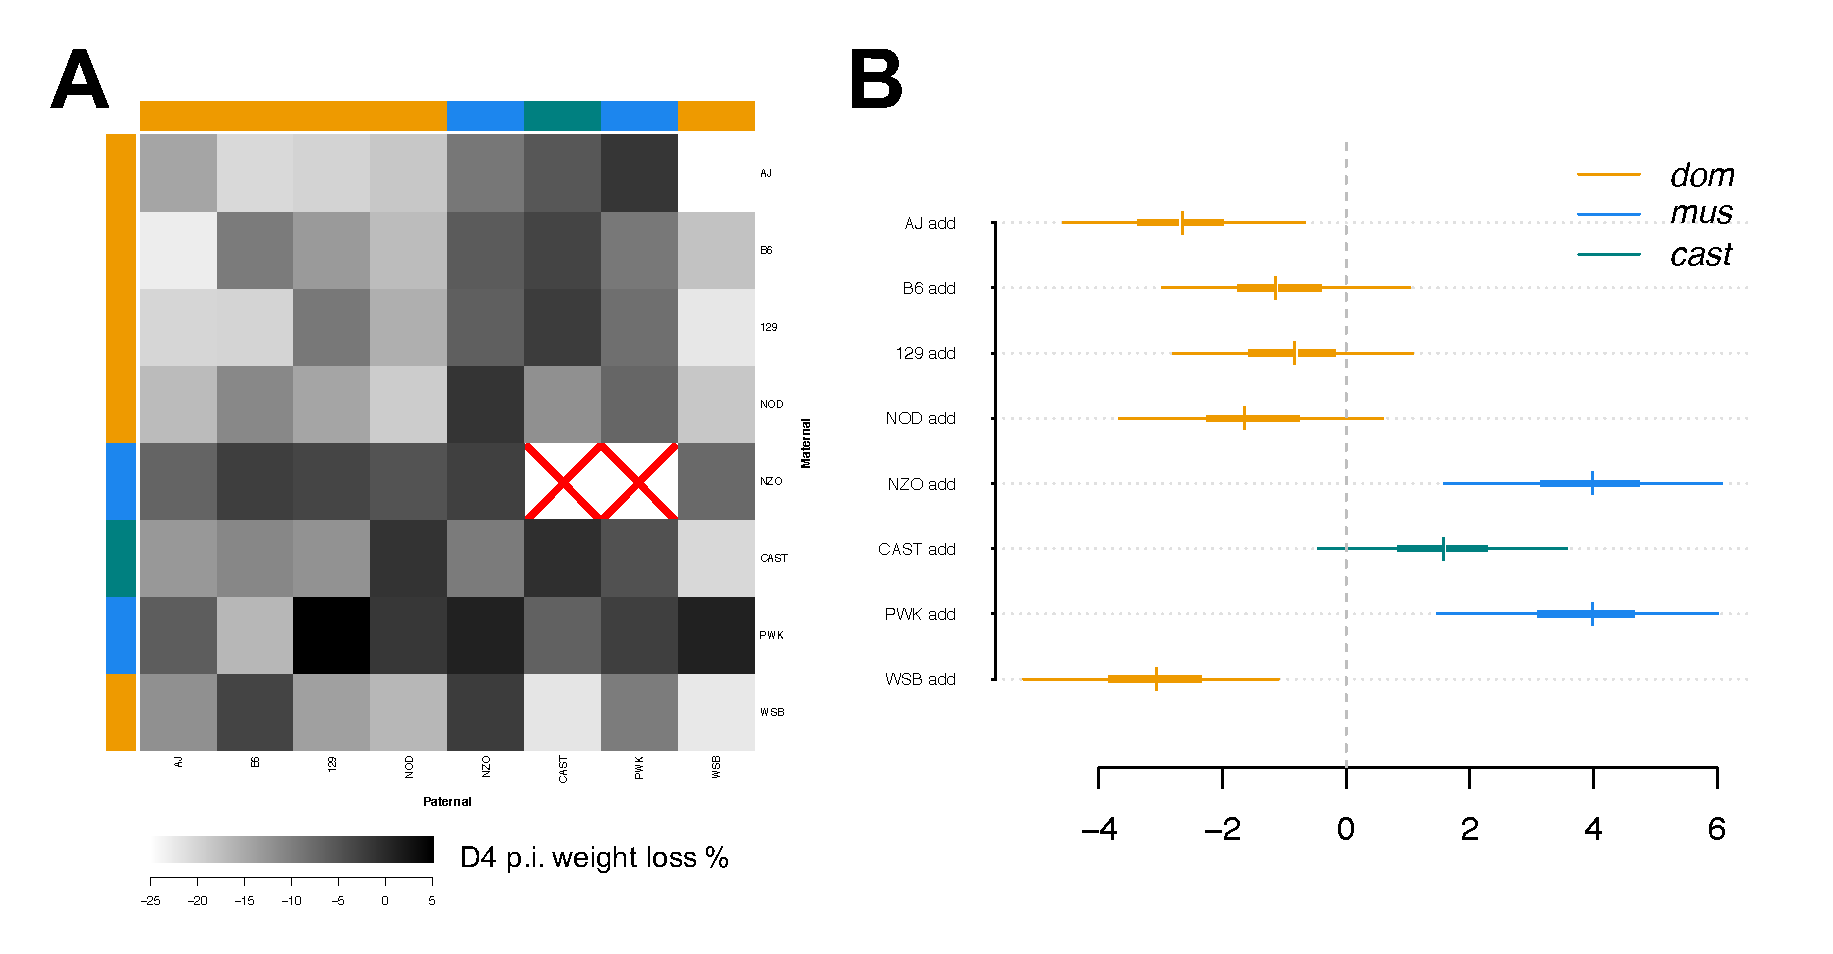
\includegraphics[width=\textwidth, trim={0in 0in 0in 0in}, clip]{figures/2-didact/flu_data_and_effects.pdf}
\caption[Response to Influenza A infection in diallel and its strain-level effects]{\textit{Mx1} as a driver of IAV-resistance can be seen in the raw data, as mean day four post-infection (D4 p.i.\ ) body weight loss percentage in a diallel of the CC founders and their hybrids (n=381 mice) (A).  Squares with a red ``X" represent crosses that produced no offspring. Resistance to IAV infection through the functional alleles of \textit{Mx1} is visible and highlighted with blue (\textit{Mx1}\textsuperscript{\textit{dom}}) and teal (\textit{Mx1}\textsuperscript{\textit{cast}}) bars. Reduced to no body weight loss is observed in mice with \textit{Mx1}\textsuperscript{\textit{dom}} (NZO and PWK) and \textit{Mx1}\textsuperscript{\textit{cast}} (CAST), reflected in the comparatively dark horizontal and vertical bars corresponding to these founders in the diallel grid. The strain-level additive effects estimated from the Bayesian hierarchical model with DIDACT reflect the possession of a functional \textit{Mx1} allele, with \textit{Mx1}\textsuperscript{\textit{dom}} (NZO and PWK) conferring more resistance than \textit{Mx1}\textsuperscript{\textit{cast}} (CAST) (B). The DIDACT-estimated strain-level additive effects are presented as highest posterior density (HPD) intervals with 95\% HPD as thin lines and 50\% HPD as thick lines, and posterior means and medians represented as colored ticks and white ticks respectively. The effects closely match those estimated in \cite{Maurizio2017}, which used the more complex BayesDiallel model, and also summarized over many imputed data sets.\label{fig:flu_data_effects}}
\end{figure}

To demonstrate a straightforward application of DIDACT to a phenotype largely driven by a single locus, we use resistance to IAV infection and the \textit{Mx1} gene. In previous work \citep{Maurizio2017}, we investigated strain-level effects in day four post-infection (D4 p.i.\ ) body weight loss percentage in a diallel of the CC founders. The phenotype of interest is a response to infection, in which three infected animals were compared to a single mock-infected animals. Occasionally three infected animals were not observed at later time points, which we accounted for through a multiple imputation procedure that imputed unobserved animals from the posterior predictive distributions of the BayesDiallel model \citep{Lenarcic2012}. Here we use only a single imputed data set of 131 outcomes, as this example is only a proof of principle for DIDACT, and not a rigorous investigation of strain-level effects. 

\subsubsection{\textit{Mx1} as a critical host-resistance factor in mice:} It has previously been shown that \textit{Mx1} largely drives IAV-resistance in the CC founders, and has three major functional classes corresponding to the three subspecies of \textit{Mus musculus}: \textit{domesticus} (hereafter \textit{dom}; CC founders with \textit{dom} allele are AJ, B6, 129, NOD, and WSB), \textit{castaneus} (\textit{cast}; CAST), and \textit{musculus} (\textit{mus}; PWK and NZO) \citep{Ferris2013}. The \textit{dom} allele of \textit{Mx1} (\textit{Mx1}\textsuperscript{\textit{dom}}) was found to be null and those individuals susceptible to IAV infection, whereas \textit{Mx1}\textsuperscript{\textit{mus}} and \textit{Mx1}\textsuperscript{\textit{cast}} confer degrees of resistance. 

Though IAV-resistance is largely Mendelian in that it is driven by \textit{Mx1}, the genetic architecture of the trait in the diallel of CC founders is more complicated than a bi-allelic locus, but rather has multiple functional alleles, \textit{Mx1}\textsuperscript{\textit{mus}} and \textit{Mx1}\textsuperscript{\textit{cast}} in comparison to the null allele \textit{Mx1}\textsuperscript{\textit{dom}}. \textit{Mx1}\textsuperscript{\textit{mus}} has a dominant mode of action, conferring the same resistance in \textit{Mx1}\textsuperscript{\textit{dom}}/\textit{Mx1}\textsuperscript{\textit{mus}} individuals as in \textit{Mx1}\textsuperscript{\textit{mus}}/\textit{Mx1}\textsuperscript{\textit{mus}}, whereas \textit{Mx1}\textsuperscript{\textit{cast}} is additive with \textit{Mx1}\textsuperscript{\textit{cast}}/\textit{Mx1}\textsuperscript{\textit{mus}} being intermediate in IAV-resistance to \textit{Mx1}\textsuperscript{\textit{mus}}/\textit{Mx1}\textsuperscript{\textit{mus}} and \textit{Mx1}\textsuperscript{\textit{cast}}/\textit{Mx1}\textsuperscript{\textit{cast}}. The increased IAV-resistance of \textit{Mx1}\textsuperscript{\textit{mus}} and \textit{Mx1}\textsuperscript{\textit{cast}} is noticeable and in the raw data and estimated strain-level effects estimated through DIDACT, highlighted in \textbf{Figure \ref{fig:flu_data_effects}}.

\subsubsection{Expectations of DIDACT with a Mendelian trait}

Our primary expectation for the performance of DIDACT with a Mendelian phenotype is that it should favor crosses that will have segregating variants at the locus, in this case \textit{Mx1}, in particular crosses that match \textit{Mx1}\textsuperscript{\textit{dom}} with \textit{Mx1}\textsuperscript{\textit{mus}} or \textit{Mx1}\textsuperscript{\textit{cast}}. Crosses that fix a homozygous genotypes at \textit{Mx1} should fix much of the trait variation, and ultimately cannot detect the Mendelian locus. As expected, DIDACT largely favors crosses that result in multiple segregating \textit{Mx1} alleles, \textit{Mx1}\textsuperscript{\textit{dom}} with \textit{Mx1}\textsuperscript{\textit{mus}} or \textit{Mx1}\textsuperscript{\textit{cast}}, shown for potential F2 experiments in \textbf{Figure \ref{fig:didact_flu_f2}} and BC experiments in \textbf{Figure \ref{fig:didact_flu_bc}}. Crosses that DIDACT predicts to be more successful than our knowledge of \textit{Mx1} would support, such as the WSB $\times$ B6 F2 cross, likely reflect effects from the genetic background of various strains that are independent of \textit{Mx1} \citep{Maurizio2017}. It is also important to note that this analysis of \textit{Mx1} represents a single imputation of the multiply imputed data. 

\begin{figure}
\renewcommand{\familydefault}{\sfdefault}\normalfont
\centering
\includegraphics[width=0.9\textwidth, page=6, trim={3.6in 0.5in 3.5in 0.5in}, clip]{figures/2-didact/mapping_crosses.pdf}
\caption[Mean posterior utility for day 4 weight loss \% post Influenza A infection in F2 crosses]{Posterior mean utility, here set to be the power to map a single QTL in 50 individuals, for the 28 possible F2 crosses of the CC founder strains. DIDACT generally estimates higher posterior mean power for F2 crosses that match a founder strain with \textit{Mx1}\textsuperscript{\textit{dom}} with either \textit{Mx1}\textsuperscript{\textit{mus}} or \textit{Mx1}\textsuperscript{\textit{cast}}, which maintains the genetic variability at \textit{Mx1} that correlates with D4 p.i.\ weight loss \%, and thus represent potentially powerful mapping crosses. F2 crosses of WSB with B6 and 129 have higher posterior mean power than other \textit{Mx1}\textsuperscript{\textit{dom}}/\textit{Mx1}\textsuperscript{\textit{dom}} pairings, likely representing the influence of other factors specific to the WSB genetic background. Posterior mean utility for BC experiments can be seen in \textbf{Figure \ref{fig:flu_data_effects}A}.\label{fig:didact_flu_f2}}
\end{figure}

\begin{figure}
\renewcommand{\familydefault}{\sfdefault}\normalfont
\centering
\includegraphics[width=0.9\textwidth, page=7, trim={3.3in 0.5in 1in 0.5in}, clip]{figures/2-didact/mapping_crosses.pdf}
\caption[Mean posterior utility for day 4 weight loss \% post Influenza A infection in BC]{Posterior mean utility, here set to be the power to map a single QTL in 50 individuals, for the 56 possible BC experiments of the CC founder strains. The A strain, corresponding to row, is the strain that is backcrossed with the F1 in the BC, therefore the homozygous genotypes of the A strain are observed along with heterozygotes. Though less obvious than in F2 crosses (\textbf{Figure \ref{fig:didact_flu_f2}}) DIDACT generally estimates higher posterior mean power for BC experiments that match a founder strain with \textit{Mx1}\textsuperscript{\textit{dom}} with either \textit{Mx1}\textsuperscript{\textit{mus}} or \textit{Mx1}\textsuperscript{\textit{cast}}, which maintains the genetic variability at \textit{Mx1} that correlates with D4 p.i.\ weight loss \%, and thus represent potentially powerful mapping crosses. BC with CAST are less powerful than NZO or PWK because \textit{Mx1}\textsuperscript{\textit{cast}} is additive in comparison to the dominance of \textit{Mx1}\textsuperscript{\textit{mus}}. BC of a strain that carries \textit{Mx1}\textsuperscript{\textit{dom}} with NZO or PWK in which the \textit{Mx1}\textsuperscript{\textit{dom}} strain is the backcrossed strain are more powerful than when either NZO or PWK are backcrossed, particularly with AJ and NOD. This is consistent with the dominant effect of \textit{Mx1}\textsuperscript{\textit{mus}}, or that \textit{Mx1}\textsuperscript{\textit{dom}}/\textit{Mx1}\textsuperscript{\textit{mus}} will be more similar to \textit{Mx1}\textsuperscript{\textit{mus}}/\textit{Mx1}\textsuperscript{\textit{mus}} in comparison to \textit{Mx1}\textsuperscript{\textit{dom}}/\textit{Mx1}\textsuperscript{\textit{mus}} to \textit{Mx1}\textsuperscript{\textit{dom}}/\textit{Mx1}\textsuperscript{\textit{dom}}.\label{fig:didact_flu_bc}}
\end{figure}

\subsection{Complex trait}

We next consider a trait that is not known to be Mendelian, but instead likely complex. 
\subsubsection{Calculated hemoglobin (cHGB):} As reported in \cite{Lenarcic2012}, blood phenotypes were measured on 626 mice, which included cHGB, an estimate of the quantity of hemoglobin in the blood (\textbf{Figure \ref{fig:chgb_figure}A}). The means of the raw data do not suggest clear strain-level effects like D4 p.i.\ weight loss \% did; however, DIDACT estimates stable strain-level effects, as well as various non-zero effects across all the effect types (\textbf{Figure \ref{fig:chgb_figure}B}). On closer inspection, the posterior utility estimates for potential experimental crosses, F2 and BC (\textbf{Figures \ref{fig:chgb_figure}C} and \textbf{\ref{fig:chgb_figure}D} respectively), correspond to the strain-level effects. For example, the strongly negative CAST inbred effect is likely responsible for DIDACT estimating higher posterior power for BC in which the CAST parent is backcrossed with the F1. DIDACT is also estimating several non-zero strain-level maternal effects, which include AJ, B6, and PWK, suggesting that RBC may have differential posterior power.

\begin{figure}
\renewcommand{\familydefault}{\sfdefault}\normalfont
\centering
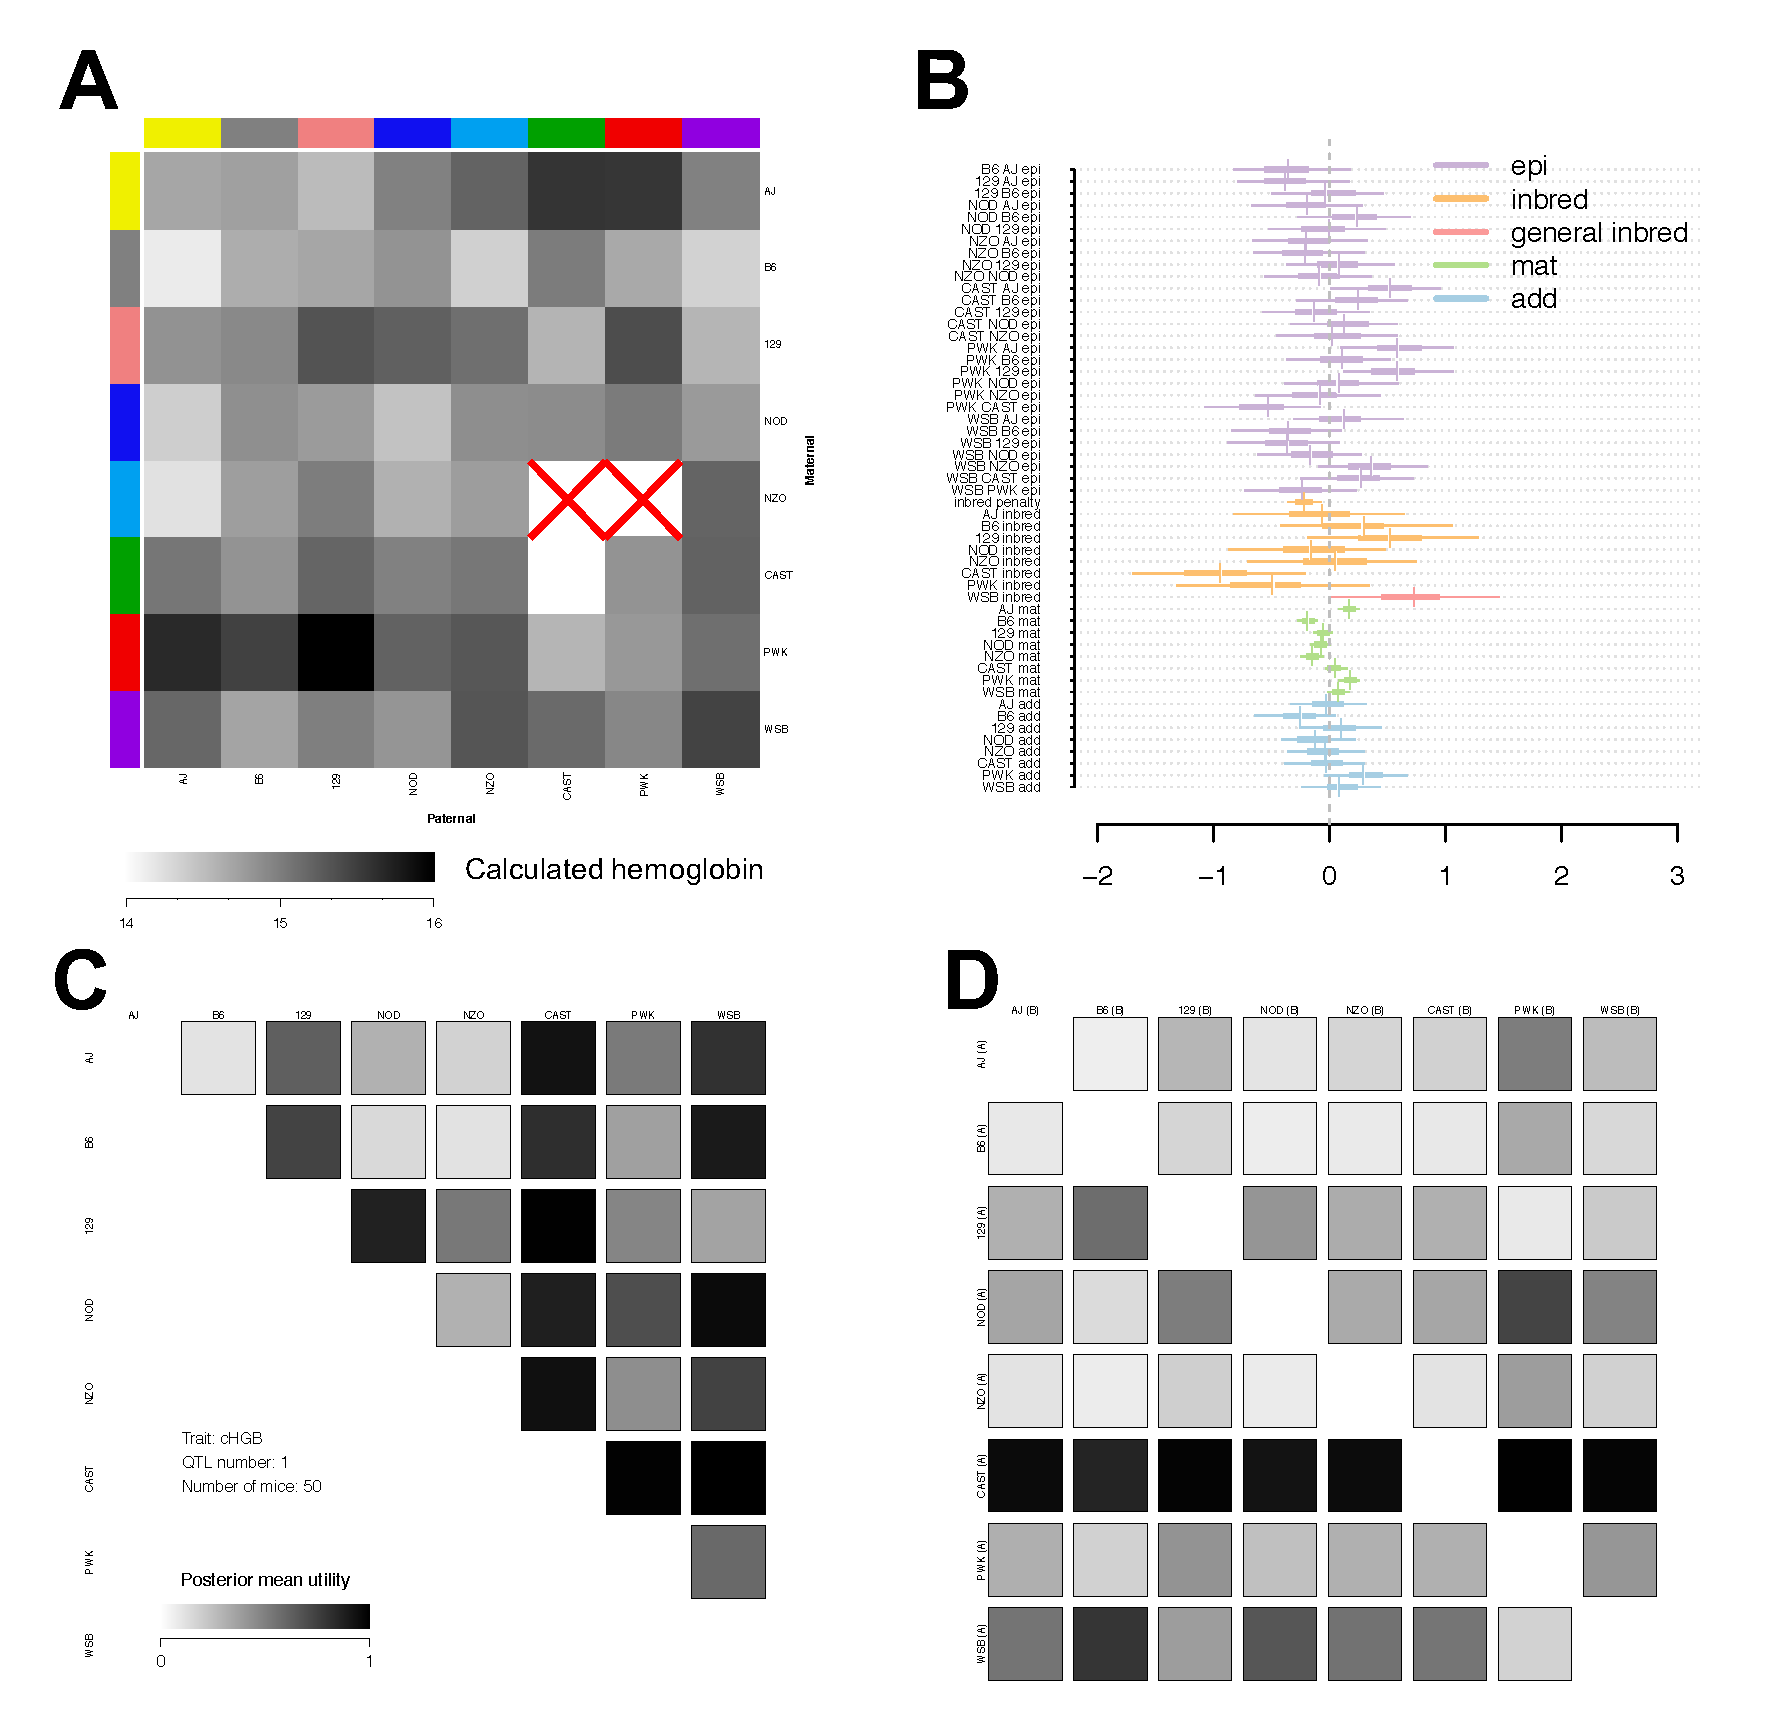
\includegraphics[width=\textwidth]{figures/2-didact/chgb_panel.pdf}
\caption[DIDACT analysis of a complex trait, calculated hemoglobin]{Calculated hemoglobin (cHGB) (g/dl) in a diallel of the CC founder strains composed of 626 mice. The cHGB diallel cell means of the raw data do not show the clear, consistent additive strain-level effects seen in the body weight response to IAV infection data (\textbf{Figure \ref{fig:flu_data_effects}A}) (A). The red ``X" represents crosses that did not produce viable offspring. Because the effects do not appear to correlate with subspecies, we use separate colors to label dam and sire strains. Despite the reduced level of visual clarity in the raw data, DIDACT is able to stably estimate strain-level effects, many of which are non-zero, and present across the various effect types (B). Effects are represented as HPD intervals, with 95\% as thin lines and 50\% as thick, and colored ticks and white ticks representing posterior means and medians respectively. This pattern of strain-level effects suggests potential complex genetic architectures underly cHGB in these strains. When DIDACT includes all of the strain-level effects into a single putative QTL effect, it results in some F2 (C) and BC (D) experiments with high posterior power. For example, the strongly negative CAST inbred effect is reflected in BC in which CAST is backcrossed having high posterior power, and low power when CAST is not backcrossed. The cHGB strain-level effects are certainly not the result of a single QTL and that assumption false, but the DIDACT results still support crosses that are likely to pair founders with highly divergent phenotypes.\label{fig:chgb_figure}}
\end{figure}

\subsection{Additional summaries of information}

DIDACT can provide more detailed descriptions of predicted bi-parental crosses than shown in \textbf{Figures \ref{fig:didact_flu_f2}}, \textbf{\ref{fig:didact_flu_bc}}, and \textbf{\ref{fig:chgb_figure}}. At its core, DIDACT is a Bayesian hierarchical model of strain-level effects that propagates uncertainty to predetermined QTL-level utility functions, and as such, posterior intervals can be produced in addition to the point estimates. Three potential F2 crosses were selected from the full panel for cHGB (\textbf{Figure \ref{fig:chgb_figure}C}), and are presented in \textbf{Figure \ref{fig:didact_chgb_detailed}}. Posterior summaries of the distribution of utility, in this case power, median utility, predicted phenotypes per QTL genotype, and variance attributable to QTL are overlayed onto the posterior mean. Unsurprisingly, DIDACT attributes higher posterior power with crosses in which the QTL explains more of the overall variability, and in which the phenotype separate more by QTL genotype.

\begin{figure}
\renewcommand{\familydefault}{\sfdefault}\normalfont
\centering
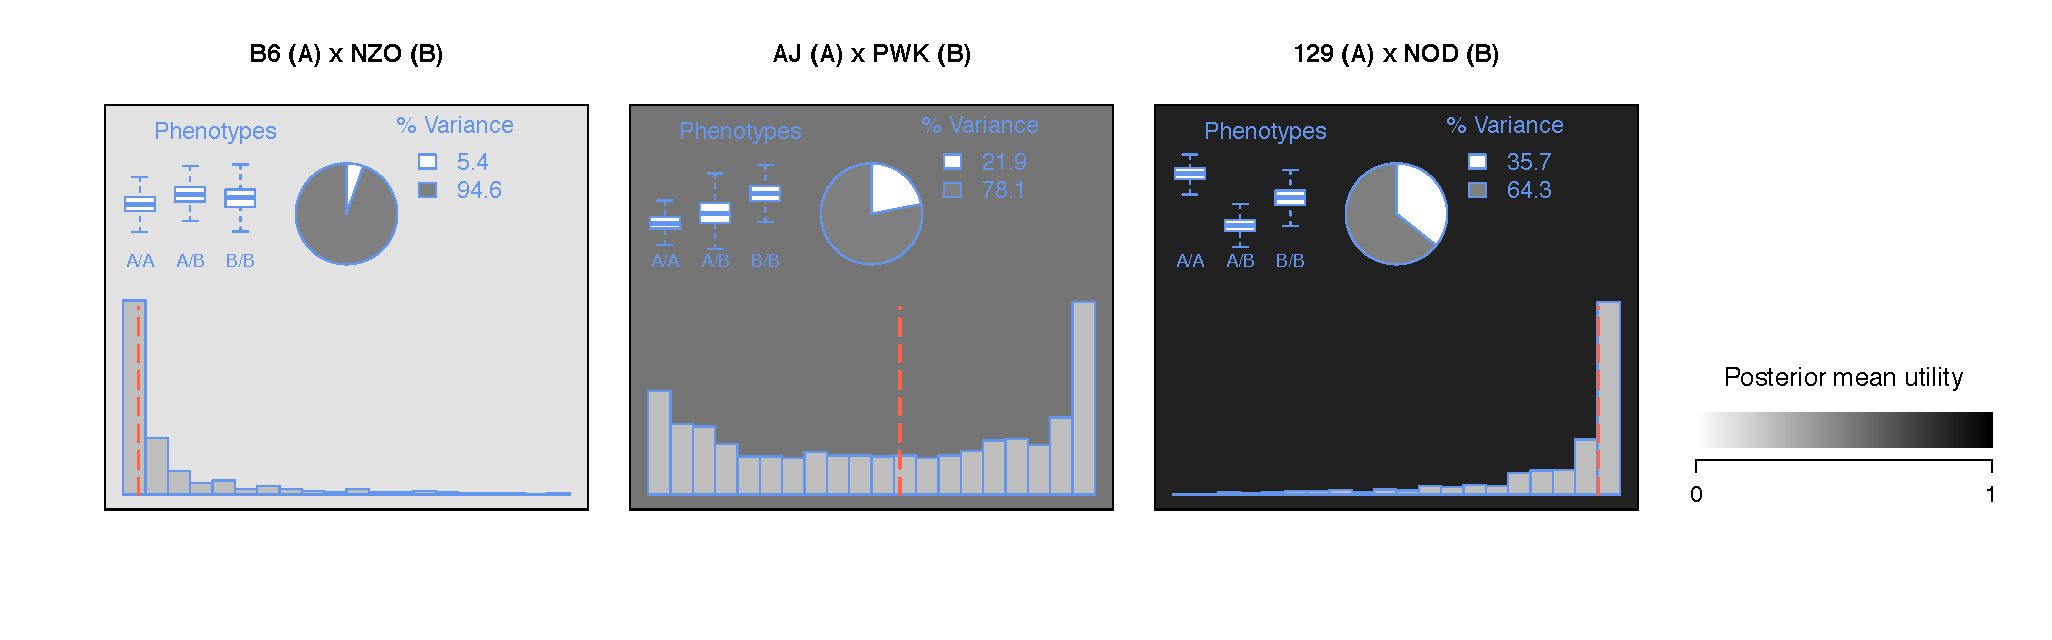
\includegraphics[width=\textwidth, trim={0.5in 0.5in 0.3in 0.2in}, clip]{figures/2-didact/DIDACT_detailed.pdf}
\caption[Detailed posterior utility visualization]{Summary plots of potential F2 crosses from DIDACT for cHGB. The full panel of potential F2 crosses are presented in \textbf{Figure \ref{fig:chgb_figure}C}. DIDACT allows for additional information to be overlayed on the posterior mean of the utility, which is represented by the background color. These plots include the histogram of the posterior distribution of the utility function, in this case power to detect a single QTL, the posterior median utility as a red dashed line, the posterior median variance explained by the QTL as a pie chart as well as point estimates, and posterior five point summaries of the phenotype per QTL genotype.\label{fig:didact_chgb_detailed}}
\end{figure}

\subsection{Parent-of-origin effects and RBC}

There is not currently a satisfactory approach and solution for parameterizing QTL effects that contain a POE mode of action, such as exists for additivity and dominance as described in Eq \ref{eq:additive} and \ref{eq:dominance} as well as in \textbf{Tables \ref{tab:qtl_mean_model}} and \textbf{\ref{tab:qtl_variance_model}}, which ultimately limits the ability of DIDACT to make power calculations for RBC as described in \textbf{Figure \ref{fig:biparental_crosses}C}. However, it is possible for DIDACT to characterize the utility in terms of predicted BC, but with the maternal and paternal identities fixed as in the RBC. Though the power calculation will not correspond to the design specified in \textbf{Figure \ref{fig:biparental_crosses}C}, in which three genetic states are observed in comparison to two for BC, differences in QTL mapping power for BC that are equivalent except for the maternal and paternal statuses of the backcrossed parental strain and F1 are potentially interesting, shown in \textbf{Figure \ref{fig:didact_chgb_rbc}} for cHGB. Corresponding BC that have markedly different posterior utility match pairings of strains with non-zero strain-level maternal effects in \textbf{Figure \ref{fig:chgb_figure}B}, such as B6 $\times$ PWK, with B6 backcrossed. For this approach to RBC, DIDACT is still dependent on assumptions connecting strain-level effects in the diallel to putative QTL segregating in a bi-parental cross; the default behavior attributes the entirety of the strain-level effects, in this case including maternal effects, to a QTL. 

\begin{figure}
\renewcommand{\familydefault}{\sfdefault}\normalfont
\centering
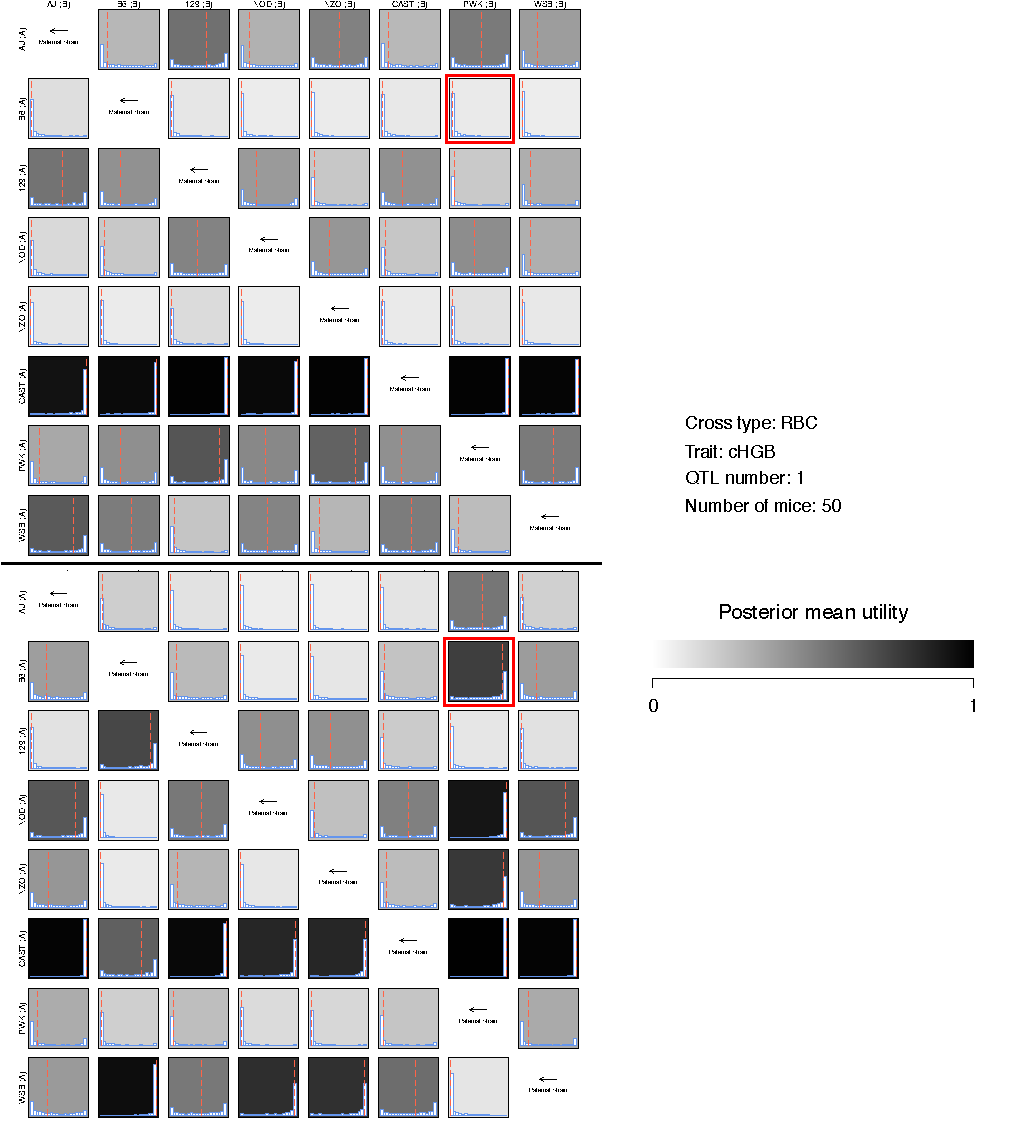
\includegraphics[width=\textwidth]{figures/2-didact/chgb_rbc_joint.pdf}
\caption[Differences in mean posterior utility due to parent-of-origin effects]{A panel of DIDACT posterior power for all possible BC in which the maternal and paternal strain identities of the F1 and backcrossed generation are fixed. Posterior histograms are included as well as posterior medians as red dashed lines. Though not a direct calculation of power for the RBC design in \textbf{Figure \ref{fig:biparental_crosses}C}, our approach highlights the potential that strain-level maternal effects can contribute to differences in predicted RBC. The B6 $\times$ PWK BC, with B6 as the backcrossed parent, are marked with red squares, for which DIDACT predicts the BC with the backcrossed B6 as the sire (lower) as being far more likely to be successful than that with a dam (upper). These predictions reflect the non-zero maternal effects estimated for B6 and PWK in \textbf{Figure \ref{fig:chgb_figure}B}. \label{fig:didact_chgb_rbc}}
\end{figure}

\section{Discussion}

We propose an experimental design approach that uses diallel data as input pilot data to characterize strain-level genetic effects with a Bayesian hierarchical model, which are then mapped with some user-defined utility function that can be used to identify promising bi-parental crosses for mapping QTL. Herein, we define utility to be QTL mapping power, though other functions could be used, so long as the strain-level effects are their inputs.

\subsection{Assumptions connecting strain-level effect to QTL effect are wrong}

DIDACT requires a strong assumption in connecting the strain-level diallel effects to putative QTL effects. We show that DIDACT performs well in a mostly Mendelian phenotype in which we can directly connect the strain-level effects to a single putative QTL. However, phenotypes that are highly heritable are often modulated through many loci, often with few or none with large effects, such as with height in humans being a clear example \citep{Wood2014}. In the vast majority of complex traits, the assumption of a single QTL absorbing all or most of the strain-level effects is wildly optimistic. However, we posit that though the assumption is unlikely, its use as a utility function can still produce a useful analysis of potential bi-parental crosses.

We make this claim because the power calculation underlying DIDACT favors QTL that explain a large proportion of the variability in the phenotype. In fact, the power function should track closely with variability explained by QTL, which will relate to the variability explained by strain identity in the diallel in this context, and could even be used as the utility function itself. Though the interpretation of the posterior utility as an accurate power may be highly unrealistic, it will select pairings that are phenotypically distinct, which is a common criterion for selecting crosses. And, it will do so in a highly principled approach that intuitively accounts for uncertainty.

\subsection{Genetic similarity between strains}

DIDACT, in its current form, does not make use of any information regarding the similarity of the inbred strains in the diallel, which could also inform how appealing an experimental cross is in terms of fine-mapping the identified QTL. The reduced complexity cross (RCC) is a developing approach in systems genetics \citep{Williams2017} in which strains that are phenotypically divergent but genetically similar are crossed, such as C57BL/6J and C57BL/6N substrains \citep{Khisti2006,Mulligan2008,Kumar2013,Simon2013,Kirkpatrick2014}. RCC provide a powerful tool for fine-mapping causal variants because the genetic variability between strains are greatly reduced, restricting the set of possible causal variants to be considered.

There are a number of ways that DIDACT could be modified to incorporate genetic similarity information, probably most simply through the utility function. The utility function could be expanded to flexibly weight potential experimental crosses by the genetic similarity, resulting in posterior utilities that are informed by both phenotype and genetic similarity. We believe this highlights the potential of DIDACT, and its underlying concept in general, to be flexible to the context of the experimental system, at the hierarchical model, but particularly at the utility function. 

\subsection{Extension to multiparental populations}

We present DIDACT analyses from diallels of the CC founders, which poses the question of designing experiments involving the CC themselves based on their diallel data. The CC are a multiparental (MPP), meaning that individuals descent from multiple well-characterized founders.  Extending the philosophy of DIDACT to experiments of an MPP RI panel is challenging, as the recombination events that randomize segments of the genome to allow for QTL mapping have already occurred during the generation of the recombinant inbred strains, and all strains have contributions from each founder at locations across the genome. Another approach to extending DIDACT to an MPP RI panel like the CC would be to consider the CC panel as a large sparse diallel, potentially with some off-diagonal cells representing F1 hybrids of the CC (CC-RIX) \citep{Bogue2015} observed. DIDACT could then be adapted to select potentially interesting but unobserved CC-RIX based on the CC-specific strain-level effects. Effectively adapting DIDACT for design of MPP experiments is an area of interest for future research.

\subsection{Summary}

We describe a novel approach to using prior collected diallel data from a panel of inbred strains to inform the selection of potential downstream experiments according to a user-specified utility function, in our case, power to map QTL in bi-parental cross experiments, consisting of F2, BC, and RBC. The core of this approach, DIDACT, is to propagate the uncertainty characterized through the Bayesian hierarchical model through to the utility functions, which can be customized to the needs and constraints of the system at hand.

As proof of principle, we evaluated DIDACT in a phenotype known to be Mendelian: resistance to IAV-infection, which is largely modulated by the \textit{Mx1} gene with a null (susceptible) and two non-null (resistant) alleles. DIDACT largely evaluated bi-parental crosses of null with non-null \textit{Mx1} strains as having higher posterior power to map the QTL. For the non-Mendelian calculated hemoglobin, DIDACT favors crosses that pair strains with contrasting phenotypes. Though the posterior power as utility, in the sense of its nominal interpretation as power, is highly optimistic, still provides a reasonable metric for comparing potential experiments, given the available pilot data. We believe our approach can be extended in many ways, in terms of both the utility function that is being optimized and the model system, many which have sparse diallel data available in the form of strain surveys. We believe DIDACT represents a philosophical advancement in terms of good experimental design and efficient use of available resources.




